\clearpage

\subsection{Opaque without Survivability}\label{ILP_Opaque_Survivability}
\begin{tcolorbox}	
\begin{tabular}{p{2.75cm} p{0.2cm} p{10.5cm}} 	
\textbf{Student Name}  &:& Tiago Esteves    (October 03, 2017 - )\\
\textbf{Goal}          &:& Implement the ILP model for the opaque transport mode without survivability.
\end{tabular}
\end{tcolorbox}

\subsubsection{Model description}

First, for a better understanding of the functions and variables used in the ILP, a table \ref{description_opaque} will be created with all indexes, inputs and variables and with their respective description.\\

\begin{table}[h!]
\centering
\begin{tabular}{ |p{1cm}||p{13cm}|}
 \hline
 \multicolumn{2}{|c|}{Description of notation used in the objective function} \\
 \hline
 \hline
 $i$ & index for start node of a physical link \\
 $j$ & index for end node of a physical link \\
 $o$ & index for node that is origin of a demand \\
 $d$ & index for node that is destination of a demand \\
 $c$ & index for bit rate of the client signal \\
 $($ i,j $)$ & physical link between the nodes $i$ and $j$ \\
 $($ o,d $)$ & demand between the nodes $o$ and $d$ \\
 $C$ & set of the client signal \\
 $f_{ij}^{od}$ & binary variable indicating if link between the nodes $i$ and $j$ is used in the path between nodes $o$ and $d$ \\
 $L_{ij}$ & binary variable indicating if link between the nodes $i$ and $j$ is used \\
 $W_{ij}$ & number of optical channels between the nodes $i$ and $j$\\
 $B_c $ & client signals granularities $($1.25, 2.5, 10, 40, 100$)$ \\
 $D_{odc}$ & client demands with bit rate $c$ between nodes $o$ and $d$ \\
 $G_{ij}$ & network topology in form of adjacency matrix \\
 \hline
\end{tabular}
\caption{Table with description of variables}
\label{description_opaque}
\end{table}

Before carrying out the description of the objective function we must take into account the following particularity of this mode of transport:
\begin{itemize}
  \item $N_{OXC,n}$ = 0, \quad $\forall$ n
  \item $N_{EXC,n}$ = 1, \quad $\forall$ n that process traffic
\end{itemize}

\vspace{11pt}
The objective function of following the ILP is a minimization of the CAPEX through the equation \ref{Capex} where in this case for the cost of nodes we only have in consideration the electric cost \ref{Capex_Node_EXC} because of the particularity previously mentioned.
In this case the value of $P_{exc,c,n}$ is obtained by equation \ref{EXC_pexc1_opaque} for long-reach and by the equation \ref{EXC_pexc2_opaque} for short-reach.\\

\newpage
As previously mentioned, equation \ref{EXC_pexc1_opaque} refers to the number of long-reach ports of the electrical switch with bit-rate -1 in node n, $P_{exc,-1,n}$, i.e. the number of line ports of node n which can be calculated as

\begin{equation}
P_{exc,-1,n} = \sum_{j=1}^{N} w_{nj}
\label{EXC_pexc1_opaque}
\end{equation}

\vspace{11pt}
where $w_{nj}$ is the number of optical channels between node $n$ and node $j$.

\vspace{11pt}
As previously mentioned, equation \ref{EXC_pexc2_opaque} refers to the number of sort-reach ports of the electrical switch with bit-rate c in node n, $P_{exc,c,n}$, i.e. the number of tributary ports with bit-rate c in node n which can be calculated as

\begin{equation}
P_{exc,c,n} = \sum_{d=1}^{N} D_{nd,c}
\label{EXC_pexc2_opaque}
\end{equation}

\vspace{11pt}
where $D_{nd,c}$ are the client demands between nodes $n$ and $d$ with bit rate $c$.

\vspace{11pt}
In this case there is the following particularity:

\begin{itemize}
  \item When $n$=$d$ the value of client demands is always zero, i.e, $D_{nn,c}=0$
\end{itemize}


\vspace{17pt}
The objective function, to be minimized, is the expression \ref{ILPOpaque_CAPEX}.\\

$subject$ $to$
\begin{equation}
\sum_{j\textbackslash \{o\}} f_{ij}^{od} = 1  \qquad \qquad \qquad \qquad \qquad \qquad \qquad \qquad \qquad \qquad
\forall(o,d) : o < d, \forall i: i = o
\label{ILPOpaque1_Surv}
\end{equation}

This constraint are equal to the constraint \ref{ILPOpaque1_CAPEX} assuming that Z variable has the value of 1.

\begin{equation}
\sum_{j\textbackslash \{o\}} f_{ij}^{od} = \sum_{j\textbackslash \{d\}} f_{ji}^{od}   \qquad \qquad \qquad \qquad \qquad \qquad \qquad \qquad
\forall(o,d) : o < d, \forall i: i \neq o,d
\label{ILPOpaque2_Surv}
\end{equation}

This constraint are equal to the constraint \ref{ILPOpaque2_CAPEX}.

\begin{equation}
\sum_{j\textbackslash \{d\}} f_{ji}^{od} = 1  \qquad \qquad \qquad \qquad \qquad \qquad \qquad \qquad \qquad \qquad
\forall(o,d) : o < d, \forall i: i = d
\label{ILPOpaque3_Surv}
\end{equation}

This constraint are equal to the constraint \ref{ILPOpaque3_CAPEX} assuming that Z variable has the value of 1.
\newpage
\begin{equation}
\sum_{o=1} \sum_{d=o+1} \left(f_{ij}^{od} + f_{ji}^{od}\right) \sum_{c\in C} (B\left(c\right) D_{odc}\leq \tau W_{ij} G_{ij} \qquad \qquad \qquad \qquad
\forall(i,j) : i < j
\label{ILPOpaque4_Surv}
\end{equation}

This restriction is considered grooming constraint, so it means the total client traffic flows can not be greater than the capacity of optical transmission system on all links where $\tau$ is always 100.

\begin{equation}
W_{ij} \leq K_{ij} L_{ij} \qquad  \qquad \qquad \qquad \qquad \qquad \qquad \qquad \qquad \qquad \qquad \qquad \forall(i,j) : i < j
\label{ILPOpaque5_Surv}
\end{equation}

This restriction concerns the capacity of the optical channels which must be less or equal to the maximum number of optical channels. For any situation the maximum number of optical channels supported by each transmission system is 100, i.e., $K_{ij}$ = 100.

\begin{equation}
f_{ij}^{od} , f_{ji}^{od} \in \{0,1\}   \qquad \qquad \qquad \qquad \qquad \qquad \qquad \qquad 
\forall(i,j) : i < j, \forall(o,d) : o < d
\label{ILPOpaque6_Surv}
\end{equation}

The number of flows per demand in this case can be zero if there are no traffic demands or one if considering traffic.

\begin{equation}
W_{ij} \in \mathbb{N}  \qquad \qquad \qquad \qquad \qquad \qquad \qquad \qquad \qquad \qquad \qquad \qquad \qquad
\forall(i,j) : i < j
\label{ILPOpaque7_Surv}
\end{equation}

The last constraint is just needed to ensure the number optical of channels is a positive integer values greater than zero.


\subsubsection{Result description}

To perform the calculations using the implementation of the models described previously it is necessary to use a mathematical software tool. For this we will use MATLAB which is ideal for dealing with linear programming problems and can call the LPsolve through an external interface.
We already have all the necessary to obtain the CAPEX value for the reference network \ref{Reference_Network_Topology}. As described in the subsection of network traffic \ref{Reference_Network_Traffic}, we have three values of network traffic (low, medium and high traffic) so we have to obtain three different CAPEX.
The value of the CAPEX of the network will be calculated based on the costs of the equipment present in the table \ref{table_cost_ilp}.\\


\textbf{Low Traffic Scenario:}\\

In this scenario we have to take into account the traffic calculated in \ref{low_scenario}. In a first phase we will show the various existing topologies of the network. The first are the allowed topologies, physical and optical topology, the second are the logical topology for all ODUs and finally the resulting physical and optical topology.\\

\newpage
\vspace{20pt}
\begin{figure}[h!]
\centering
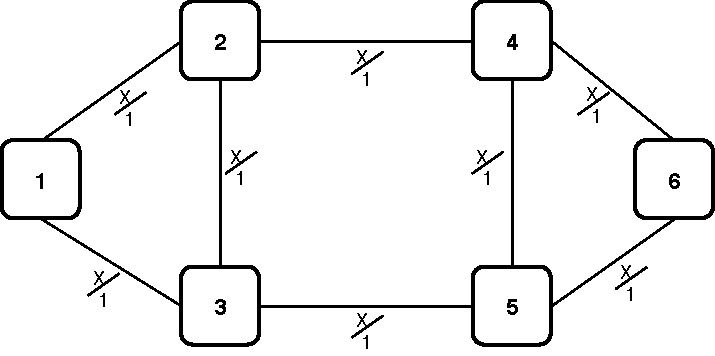
\includegraphics[width=13cm]{sdf/ilp/opaque_survivability/figures/allowed_physical_topology}
\caption{Allowed Physical Topology. The allowed physical topology is defined by the duct and sites in the field. It is assumed that each duct supports up to 1 bidirectional transmission system and each site supports up to 1 node.}
\label{allowed_physical_low}
\end{figure}

\vspace{20pt}
\begin{figure}[h!]
\centering
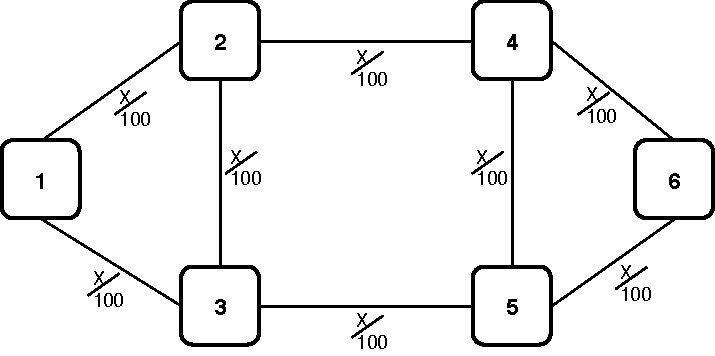
\includegraphics[width=13cm]{sdf/ilp/opaque_survivability/figures/allowed_optical_topology}
\caption{Allowed Optical Topology. The allowed optical topology is defined by the transport mode (opaque transport mode in this case). It is assumed that each transmission system supports up to 100 optical channels.}
\label{allowed_optical_low}
\end{figure}

\newpage
\begin{figure}[h!]
\centering
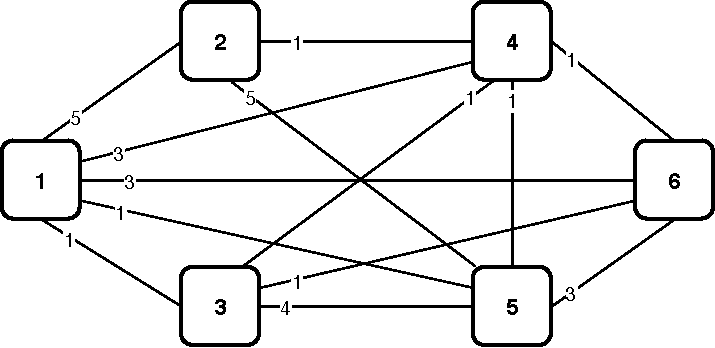
\includegraphics[width=12cm]{sdf/ilp/opaque_survivability/figures/logical_topology_ODU0_low}
\caption{ODU0 Logical Topology defined by the ODU0 traffic matrix.}
\label{logical_ODU0_low}
\end{figure}

\begin{figure}[h!]
\centering
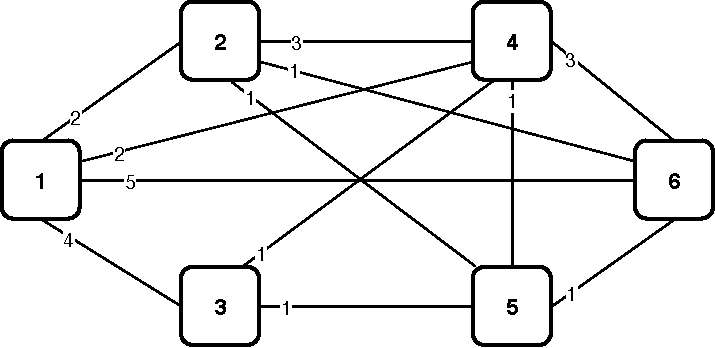
\includegraphics[width=12cm]{sdf/ilp/opaque_survivability/figures/logical_topology_ODU1_low}
\caption{ODU1 Logical Topology defined by the ODU1 traffic matrix.}
\label{logical_ODU1_low}
\end{figure}

\begin{figure}[h!]
\centering
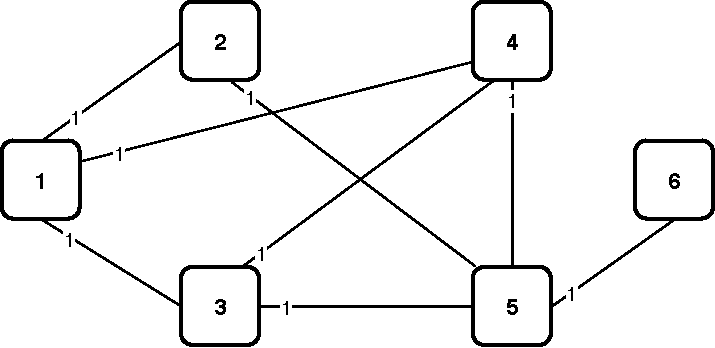
\includegraphics[width=12cm]{sdf/ilp/opaque_survivability/figures/logical_topology_ODU2_low}
\caption{ODU2 Logical Topology defined by the ODU2 traffic matrix.}
\label{logical_ODU2_low}
\end{figure}

\begin{figure}[h!]
\centering
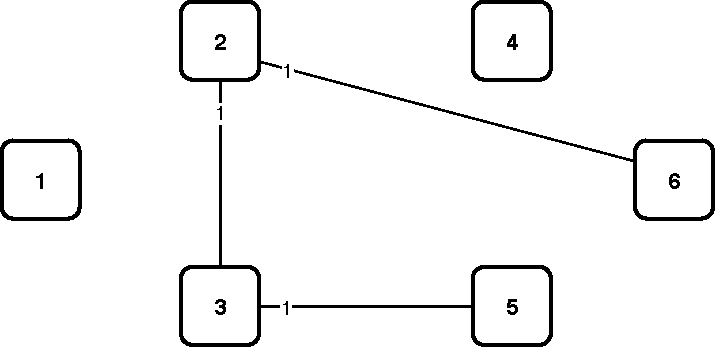
\includegraphics[width=12cm]{sdf/ilp/opaque_survivability/figures/logical_topology_ODU3_low}
\caption{ODU3 Logical Topology defined by the ODU3 traffic matrix.}
\label{logical_ODU3_low}
\end{figure}

\begin{figure}[h!]
\centering
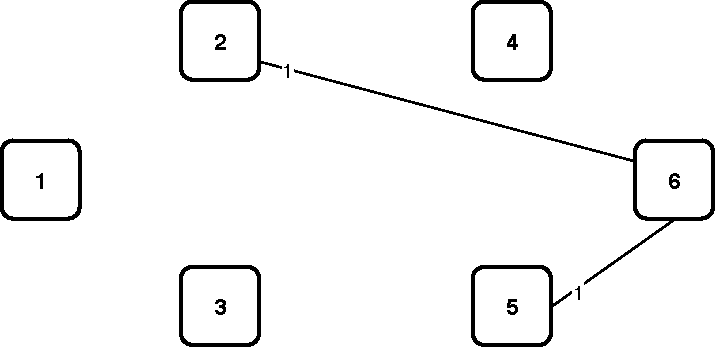
\includegraphics[width=12cm]{sdf/ilp/opaque_survivability/figures/logical_topology_ODU4_low}
\caption{ODU4 Logical Topology defined by the ODU4 traffic matrix.}
\label{logical_ODU4_low}
\end{figure}

\begin{figure}[h!]
\centering
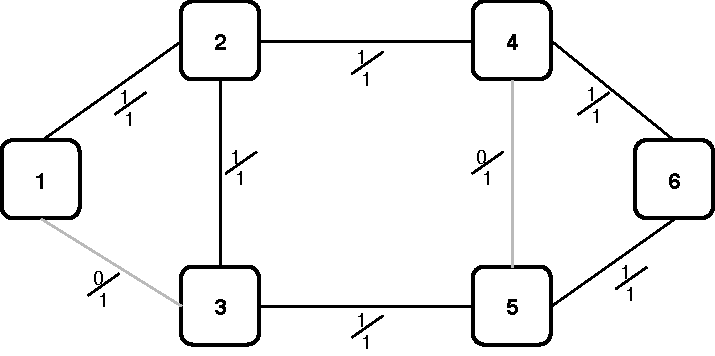
\includegraphics[width=12cm]{sdf/ilp/opaque_survivability/figures/physical_topology_low}
\caption{Physical Topology after dimensioning.}
\label{physical_low}
\end{figure}

\begin{figure}[h!]
\centering
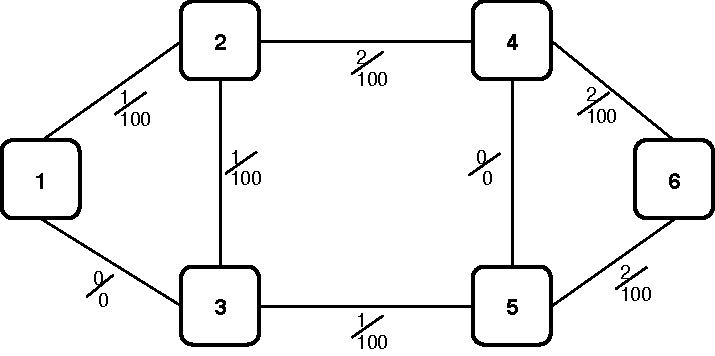
\includegraphics[width=13cm]{sdf/ilp/opaque_survivability/figures/optical_topology_low}
\caption{Optical Topology after dimensioning.}
\label{optical_low}
\end{figure}

\vspace{15pt}
In table \ref{link_opaque_surv_ref_low} we can see the number of optical channels calculated using \ref{Capex_Link} and \ref{ILPOpaque_CAPEX} and the number of amplifiers for each link calculated using \ref{Capex_amplifiers}.\\

\begin{table}[h!]
\centering
\begin{tabular}{|| c | c | c ||}
 \hline
 \multicolumn{3}{|| c ||}{Information regarding links} \\
 \hline
 \hline
 Bidirectional Link & Optical Channels & Amplifiers\\
 \hline
 Node 1 <-> Node 2 & 1 & 4 \\
 Node 1 <-> Node 3 & 0 & 6 \\
 Node 2 <-> Node 3 & 1 & 0 \\
 Node 2 <-> Node 4 & 2 & 6 \\
 Node 3 <-> Node 5 & 1 & 8 \\
 Node 4 <-> Node 5 & 0 & 1 \\
 Node 4 <-> Node 6 & 2 & 7 \\
 Node 5 <-> Node 6 & 2 & 3 \\
 \hline
\end{tabular}
\caption{Table with information regarding links}
\label{link_opaque_surv_ref_low}
\end{table}

\vspace{15pt}
In table \ref{node_opaque_surv_ref_low} we can see the resulting nodal degree at the physical layer, the number of line ports and the number of tributary ports for each node.\\
\newpage
\begin{table}[h!]
\centering
\begin{tabular}{|| c | c | c | c ||}
 \hline
 \multicolumn{4}{|| c ||}{Information regarding nodes} \\
 \hline
 \hline
 Node & Resulting Nodal Degree & Line Ports & Tributary Ports\\
 \hline
 1 & 1 & 1 & 29 \\
 2 & 3 & 4 & 23 \\
 3 & 2 & 2 & 18 \\
 4 & 2 & 4 & 20 \\
 5 & 2 & 3 & 24 \\
 6 & 2 & 4 & 22 \\
\hline
\end{tabular}
\caption{Table with information regarding nodes}
\label{node_opaque_surv_ref_low}
\end{table}

Through the information obtained previously on the nodes we can now create tables with detailed information about each node. In each table mentioned below we can see how many ports are connected to a given node and its bit rate (in relation to the line ports) and how many ports are assigned to each different bit rate (in relation to the tributary ports).\\

\begin{table}[h!]
\centering
\begin{tabular}{|| c | c | c ||}
 \hline
 \multicolumn{3}{|| c ||}{Detailed description of Node 1} \\
 \hline
 \hline
  & Node<--Optical Channels-->Node & Bit rate \\
 \hline
 1 line ports & 1  <---- 1 ---->  2 & 100 Gbits/s \\
 \hline
 \hline
  & Number of tributary ports & Bit rate \\ \hline
\multirow{3}{*}{29 tributary ports} & 13 & ODU0 \\
 & 13 & ODU1 \\
 & 3 & ODU2 \\
\hline
\end{tabular}
\caption{Table with detailed description of node 1}
\end{table}

\vspace{13pt}
\begin{table}[h!]
\centering
\begin{tabular}{|| c | c | c ||}
 \hline
 \multicolumn{3}{|| c ||}{Detailed description of Node 2} \\
 \hline
 \hline
  & Node<--Optical Channels-->Node & Bit rate \\ \hline
 \multirow{3}{*}{4 line ports} & 2  <---- 1 ---->  1 & \multirow{3}{*}{100 Gbits/s} \\
 & 2  <---- 1 ---->  3 & \\
 & 2  <---- 2 ---->  4 & \\
 \hline
 \hline
  & Number of tributary ports & Bit rate \\ \hline
\multirow{5}{*}{23 tributary ports} & 11 & ODU0 \\
 & 7 & ODU1 \\
 & 2 & ODU2 \\
 & 2 & ODU3 \\
 & 1 & ODU4 \\
\hline
\end{tabular}
\caption{Table with detailed description of node 2}
\end{table}

\newpage
\begin{table}[h!]
\centering
\begin{tabular}{|| c | c | c ||}
 \hline
 \multicolumn{3}{|| c ||}{Detailed description of Node 3} \\
 \hline
 \hline
  & Node<--Optical Channels-->Node & Bit rate \\
 \hline
 \multirow{2}{*}{2 line ports} & 3  <---- 1 ---->  2 & \multirow{2}{*}{100 Gbits/s}\\
 & 3  <---- 1 ---->  5 & \\
 \hline
 \hline
  & Number of tributary ports & Bit rate \\ \hline
\multirow{4}{*}{18 tributary ports} & 7 & ODU0 \\
 & 6 & ODU1\\
 & 3 & ODU2\\
 & 2 & ODU3\\
\hline
\end{tabular}
\caption{Table with detailed description of node 3}
\end{table}

\vspace{13pt}
\begin{table}[h!]
\centering
\begin{tabular}{|| c | c | c ||}
 \hline
 \multicolumn{3}{|| c ||}{Detailed description of Node 4} \\
 \hline
 \hline
  & Node<--Optical Channels-->Node & Bit rate \\
 \hline
 \multirow{2}{*}{4 line ports} & 4  <---- 2 ---- >  2 & \multirow{2}{*}{100 Gbits/s}\\
 & 4  <---- 2 ----> 6 & \\
 \hline
 \hline
  & Number of tributary ports & Bit rate \\ \hline
\multirow{3}{*}{20 tributary ports} & 7 & ODU0 \\
 & 10 & ODU1 \\
 & 3 & ODU2 \\
\hline
\end{tabular}
\caption{Table with detailed description of node 4}
\end{table}

\vspace{13pt}
\begin{table}[h!]
\centering
\begin{tabular}{|| c | c | c ||}
 \hline
 \multicolumn{3}{|| c ||}{Detailed description of Node 5} \\
 \hline
 \hline
  & Node<--Optical Channels-->Node & Bit rate \\
 \hline
 \multirow{2}{*}{3 line ports} & 5  <---- 1 ---->  3 & \multirow{2}{*}{100 Gbits/s}\\
 & 5  <---- 2 ---->  6 & \\
 \hline
 \hline
  & Number of tributary ports & Bit rate \\ \hline
\multirow{5}{*}{24 tributary ports} & 14 & ODU0 \\
 & 4 & ODU1 \\
 & 4 & ODU2 \\
 & 1 & ODU3 \\
 & 1 & ODU4 \\
\hline
\end{tabular}
\caption{Table with detailed description of node 5}
\end{table}

\newpage
\begin{table}[h!]
\centering
\begin{tabular}{|| c | c | c ||}
 \hline
 \multicolumn{3}{|| c ||}{Detailed description of Node 6} \\
 \hline
 \hline
  & Node<--Optical Channels-->Node & Bit rate \\
 \hline
 \multirow{2}{*}{4 line ports} & 6  <---- 2 ---->  4 & \multirow{2}{*}{100 Gbits/s}\\
 & 6  <---- 2 ---->  5 & \\
 \hline
 \hline
  & Number of tributary ports & Bit rate \\ \hline
\multirow{5}{*}{22 tributary ports} & 8 & ODU0 \\
 & 10 & ODU1 \\
 & 1 & ODU2 \\
 & 1 & ODU3 \\
 & 2 & ODU4 \\
\hline
\end{tabular}
\caption{Table with detailed description of node 6}
\end{table}

\vspace{17pt}
Now through the table \ref{scriptopaque_surv_ref_low} we can see the result of CAPEX obtained with this ILP model.\\

\begin{table}[h!]
\centering
\begin{tabular}{|| c | c | c | c | c | c | c ||}
 \hline
 \multicolumn{7}{|| c ||}{CAPEX of the Network} \\
 \hline
 \hline
 \multicolumn{3}{|| c |}{ } & Quantity & Unit Price & Cost & Total \\
 \hline
 \multirow{3}{*}{Link Cost} & \multicolumn{2}{ c |}{OLTs} & 12 & 15 000 \euro & 180 000 \euro & \multirow{3}{*}{9 404 000 \euro} \\ \cline{2-6}
 & \multicolumn{2}{ c |}{100 Gb/s Transceivers} & 18 & 5 000 \euro/Gb/s & 9 000 000 \euro & \\ \cline{2-6}
 & \multicolumn{2}{ c |}{Amplifiers} & 56 & 4 000 \euro & 224 000 \euro & \\
 \hline
 \multirow{9}{*}{Node Cost} & \multirow{7}{*}{Electrical} & EXCs & 6 & 10 000 \euro & 60 000 \euro & \multirow{9}{*}{1 862 590 \euro} \\ \cline{3-6}
 & & ODU0 Ports & 60 & 10 \euro/port & 600 \euro & \\ \cline{3-6}
 & & ODU1 Ports & 50 & 15 \euro/port & 750 \euro & \\ \cline{3-6}
 & & ODU2 Ports & 16 & 30 \euro/port & 480 \euro & \\ \cline{3-6}
 & & ODU3 Ports & 6 & 60 \euro/port & 360 \euro & \\ \cline{3-6}
 & & ODU4 Ports & 4 & 100 \euro/port & 400 \euro & \\ \cline{3-6}
 & & Line Ports & 18 & 100 000 \euro/port & 1 800 000 \euro & \\ \cline{2-6}
 & \multirow{2}{*}{Optical} & OXCs & 0 & 20 000 \euro & 0 \euro & \\ \cline{3-6}
 & & Ports & 0 & 2 500 \euro/port & 0 \euro & \\
 \hline
 \multicolumn{6}{|| c |}{Total Network Cost} & 11 266 590 \euro \\
\hline
\end{tabular}
\caption{Table with detailed description of CAPEX}
\label{scriptopaque_surv_ref_low}
\end{table}

\newpage
All the values calculated in the previous table were obtained through the equations \ref{Capex_Link} and \ref{Capex_Node} referred to in section \ref{ILP_CAPEX}, but for a more detailed analysis we created table \ref{formulas_opaque_surv_ref_low} where we can see how all the parameters are calculated individually.\\

\begin{table}[h!]
\centering
\begin{tabular}{|| c | c ||}
 \hline
  & Equation used to calculate the cost \\ \hline
 OLTs & \(\displaystyle 2 \sum_{i=1}^{N}\sum_{j=i+1}^{N} L_{ij} \gamma_0^{OLT} \) \\ \hline
 Transceivers & \(\displaystyle 2 \sum_{i=1}^{N}\sum_{j=i+1}^{N} L_{ij} W_{ij} \gamma_1^{OLT} \tau \) \\ \hline
 Amplifiers & \(\displaystyle 2 \sum_{i=1}^{N}\sum_{j=i+1}^{N} L_{ij} N^R_{ij} c^R \) \\ \hline
 EXCs & \(\displaystyle \sum_{n=1}^N N_{exc,n} \gamma_{e0} \) \\ \hline
 ODU0 & \(\displaystyle \sum_{n=1}^{N} \sum_{d=1}^{N} N_{exc,n} D_{nd,0} \gamma_{e1,0} \) \\ \hline
 ODU1 & \(\displaystyle \sum_{n=1}^{N} \sum_{d=1}^{N} N_{exc,n} D_{nd,1} \gamma_{e1,1} \) \\ \hline
 ODU2 & \(\displaystyle \sum_{n=1}^{N} \sum_{d=1}^{N} N_{exc,n} D_{nd,2} \gamma_{e1,2} \)\\ \hline
 ODU3 & \(\displaystyle \sum_{n=1}^{N} \sum_{d=1}^{N} N_{exc,n} D_{nd,3} \gamma_{e1,3} \) \\ \hline
 ODU4 & \(\displaystyle \sum_{n=1}^{N} \sum_{d=1}^{N} N_{exc,n} D_{nd,4} \gamma_{e1,4} \) \\ \hline
 Line & \(\displaystyle \sum_{n=1}^{N} \sum_{j=1}^{N} N_{exc,n} w_{nj} \gamma_{e1,-1} \) \\ \hline
 OXCs & For opaque transport mode this parameter is always zero. \\ \hline
 $P_{oxc}$ & Does not exist for this case then it is equal to zero. \\ \hline
 CAPEX & The final cost is calculated by summing all previous results. \\
 \hline
 \end{tabular}
\caption{Table with description of calculation}
\label{formulas_opaque_surv_ref_low}
\end{table}

\vspace{17pt}
Finally let's focus on the routing information. These paths are bidirectional so the path from one node to another is the same path in the opposite direction. In table \ref{path_opaque_surv_ref_low} we can see all the routing obtained for all nodes.\\
\newpage
\begin{table}[h!]
\centering
\begin{tabular}{|| c | c | c ||}
 \hline
 \multicolumn{3}{|| c ||}{Routing} \\
 \hline
 \hline
 o & d & Links \\
 \hline
 1 & 2 & \{(1,2)\} \\ \hline
 1 & 3 & \{(1,2),(2,3)\} \\ \hline
 1 & 4 & \{(1,2),(2,4)\}\\ \hline
 1 & 5 & \{(1,2),(2,3),(3,5)\}\\ \hline
 1 & 6 & \{(1,2),(2,4),(4,6)\}\\ \hline
 2 & 3 & \{(2,3)\}\\ \hline
 2 & 4 & \{(2,4)\}\\ \hline
 2 & 5 & \{(2,3),(3,5)\}\\ \hline
 2 & 6 & \{(2,4),(4,6)\}\\ \hline
 3 & 4 & \{(3,2),(2,4)\}\\ \hline
 3 & 5 & \{(3,5)\}\\ \hline
 3 & 6 & \{(3,5),(5,6)\}\\ \hline
 4 & 5 & \{(4,6),(6,5)\}\\ \hline
 4 & 6 & \{(4,6)\}\\ \hline
 5 & 6 & \{(5,6)\}\\
 \hline
\end{tabular}
\caption{Table with description of routing}
\label{path_opaque_surv_ref_low}
\end{table}

\vspace{13pt}
\textbf{Medium Traffic Scenario:}\\

In this scenario we have to take into account the traffic calculated in \ref{medium_traffic_scenario}. In a first phase we will show the various existing topologies of the network. \\

\begin{figure}[h!]
\centering
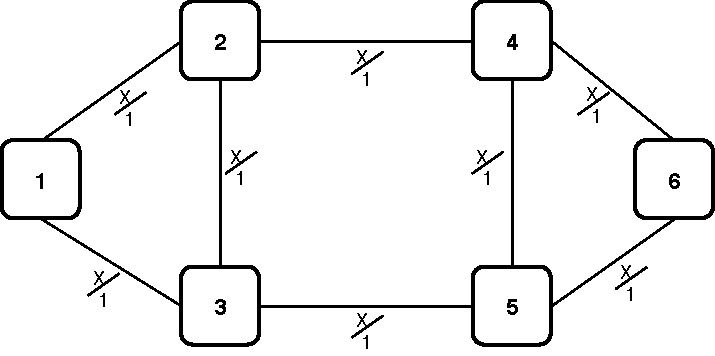
\includegraphics[width=12cm]{sdf/ilp/opaque_survivability/figures/allowed_physical_topology}
\caption{Allowed Physical Topology. The allowed physical topology is defined by the duct and sites in the field. It is assumed that each duct supports up to 1 bidirectional transmission system and each site supports up to 1 node.}
\label{allowed_physical_medium}
\end{figure}

\begin{figure}[h!]
\centering
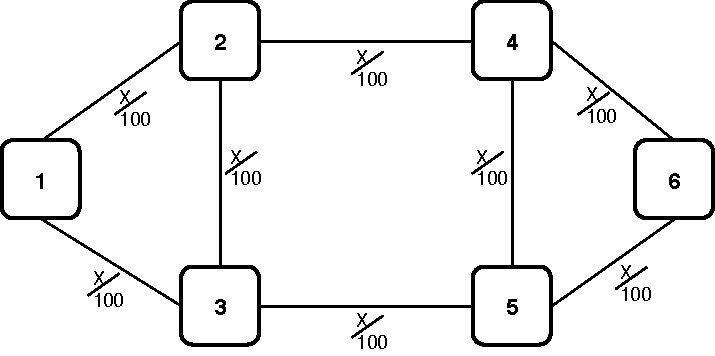
\includegraphics[width=11cm]{sdf/ilp/opaque_survivability/figures/allowed_optical_topology}
\caption{Allowed Optical Topology. The allowed optical topology is defined by the transport mode (opaque transport mode in this case). It is assumed that each transmission system supports up to 100 optical channels.}
\label{allowed_optical_medium}
\end{figure}

\begin{figure}[h!]
\centering
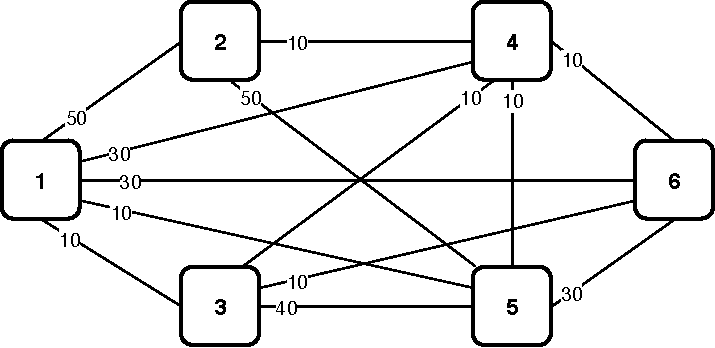
\includegraphics[width=11cm]{sdf/ilp/opaque_survivability/figures/logical_topology_ODU0_medium}
\caption{ODU0 Logical Topology defined by the ODU0 traffic matrix.}
\label{logical_ODU0_medium}
\end{figure}

\begin{figure}[h!]
\centering
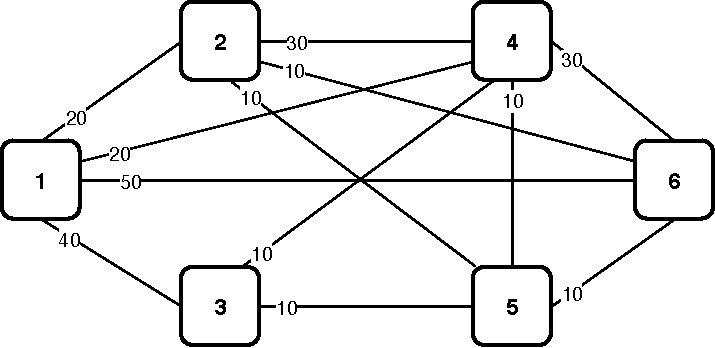
\includegraphics[width=12cm]{sdf/ilp/opaque_survivability/figures/logical_topology_ODU1_medium}
\caption{ODU1 Logical Topology defined by the ODU1 traffic matrix.}
\label{logical_ODU1_medium}
\end{figure}

\begin{figure}[h!]
\centering
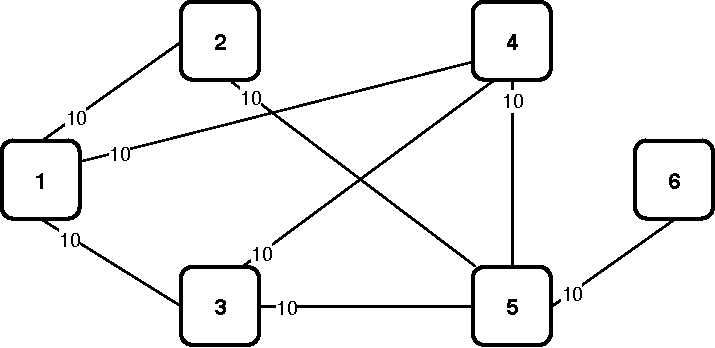
\includegraphics[width=12cm]{sdf/ilp/opaque_survivability/figures/logical_topology_ODU2_medium}
\caption{ODU2 Logical Topology defined by the ODU2 traffic matrix.}
\label{logical_ODU2_medium}
\end{figure}

\begin{figure}[h!]
\centering
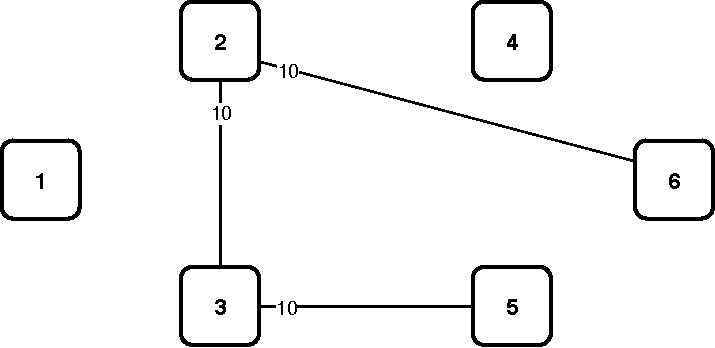
\includegraphics[width=12cm]{sdf/ilp/opaque_survivability/figures/logical_topology_ODU3_medium}
\caption{ODU3 Logical Topology defined by the ODU3 traffic matrix.}
\label{logical_ODU3_medium}
\end{figure}

\begin{figure}[h!]
\centering
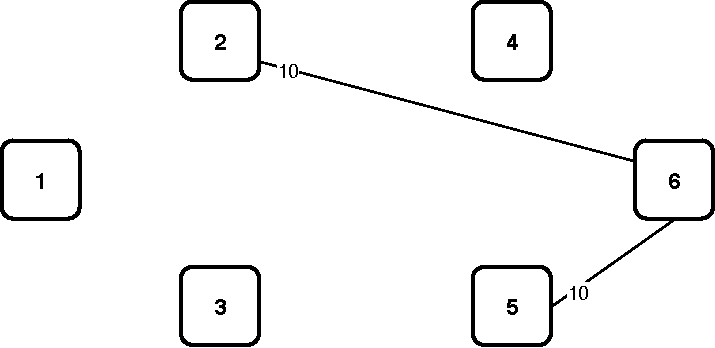
\includegraphics[width=12cm]{sdf/ilp/opaque_survivability/figures/logical_topology_ODU4_medium}
\caption{ODU4 Logical Topology defined by the ODU4 traffic matrix.}
\label{logical_ODU4_medium}
\end{figure}
\newpage
\begin{figure}[h!]
\centering
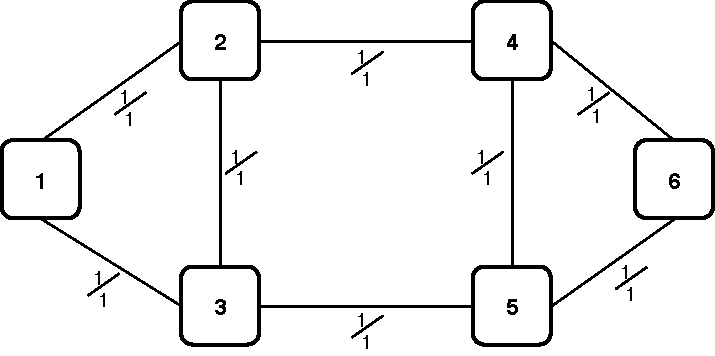
\includegraphics[width=13cm]{sdf/ilp/opaque_survivability/figures/physical_topology}
\caption{Physical Topology after dimensioning.}
\label{physical_medium}
\end{figure}

\begin{figure}[h!]
\centering
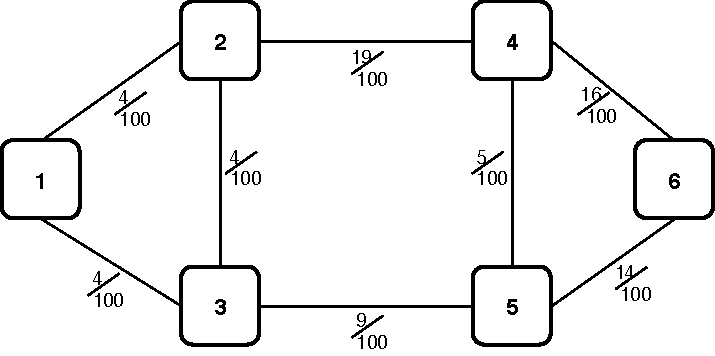
\includegraphics[width=13cm]{sdf/ilp/opaque_survivability/figures/optical_topology_medium}
\caption{Optical Topology after dimensioning.}
\label{optical_medium}
\end{figure}

\vspace{17pt}
In table \ref{link_opaque_surv_ref_medium} we can see the number of optical channels calculated using \ref{Capex_Link} and \ref{Capex} and the number of amplifiers for each link calculated using \ref{Capex_amplifiers}.\\

In table \ref{node_opaque_surv_ref_medium} we can see the resulting nodal degree at the physical layer, the number of line ports and the number of tributary ports for each node.\\
\newpage
\begin{table}[h!]
\centering
\begin{tabular}{|| c | c | c ||}
 \hline
 \multicolumn{3}{|| c ||}{Information regarding links} \\
 \hline
 \hline
 Bidirectional Link & Optical Channels & Amplifiers\\
 \hline
 Node 1 <-> Node 2 & 4 & 4 \\
 Node 1 <-> Node 3 & 4 & 6 \\
 Node 2 <-> Node 3 & 4 & 0 \\
 Node 2 <-> Node 4 & 19 & 6 \\
 Node 3 <-> Node 5 & 9 & 8 \\
 Node 4 <-> Node 5 & 5 & 1 \\
 Node 4 <-> Node 6 & 16 & 7 \\
 Node 5 <-> Node 6 & 14 & 3 \\
 \hline
\end{tabular}
\caption{Table with information regarding links}
\label{link_opaque_surv_ref_medium}
\end{table}

\begin{table}[h!]
\centering
\begin{tabular}{|| c | c | c | c ||}
 \hline
 \multicolumn{4}{|| c ||}{Information regarding nodes} \\
 \hline
 \hline
 Node & Resulting Nodal Degree & Line Ports & Tributary Ports\\
 \hline
 1 & 2 & 8 & 290 \\
 2 & 3 & 27 & 230 \\
 3 & 3 & 17 & 180 \\
 4 & 3 & 40 & 200 \\
 5 & 3 & 28 & 240 \\
 6 & 2 & 30 & 220 \\
\hline
\end{tabular}
\caption{Table with information regarding nodes}
\label{node_opaque_surv_ref_medium}
\end{table}

Through the information obtained previously on the nodes we can now create tables with detailed information about each node.
In each table with detailed information we can see how many ports are connected to a given node and its bit rate (in relation to the line ports) and how many ports are assigned to each different bit rate (in relation to the tributary ports).\\

\begin{table}[h!]
\centering
\begin{tabular}{|| c | c | c ||}
 \hline
 \multicolumn{3}{|| c ||}{Detailed description of Node 1} \\
 \hline
 \hline
  & Node <-- Optical Channels --> Node & bit rate \\ \hline
\multirow{2}{*}{8 line ports} & 1  <---- 4 ---->  2 & \multirow{2}{*}{100 Gbtis/s} \\
 & 1  <---- 4 ----> 3 & \\
 \hline
 \hline
  & Number of tributary ports & bit rate \\ \hline
\multirow{3}{*}{290 tributary ports} & 130 & ODU0 \\
 & 130 & ODU1 \\
 & 30 & ODU2 \\
\hline
\end{tabular}
\caption{Table with detailed description of node 1}
\end{table}

\newpage
\begin{table}[h!]
\centering
\begin{tabular}{|| c | c | c ||}
 \hline
 \multicolumn{3}{|| c ||}{Detailed description of Node 2} \\
 \hline
 \hline
  & Node <-- Optical Channels --> Node & bit rate \\ \hline
 \multirow{3}{*}{27 line ports} & 2  <---- 4 ---->  1 & \multirow{3}{*}{100 Gbtis/s}\\
 & 2  <---- 4 ---->  3 & \\
 & 2  <---- 19 ---->  4 & \\
 \hline
 \hline
  & Number of tributary ports & bit rate \\ \hline
\multirow{5}{*}{230 tributary ports} & 110 & ODU0 \\
 & 70 & ODU1 \\
 & 20 & ODU2 \\
 & 20 & ODU3 \\
 & 10 & ODU4 \\
\hline
\end{tabular}
\caption{Table with detailed description of node 2}
\end{table}

\vspace{17pt}
\begin{table}[h!]
\centering
\begin{tabular}{|| c | c | c ||}
 \hline
 \multicolumn{3}{|| c ||}{Detailed description of Node 3} \\
 \hline
 \hline
  & Node <-- Optical Channels --> Node & bit rate \\ \hline
 \multirow{3}{*}{17 line ports} & 3  <---- 4 ---->  1 & \multirow{3}{*}{100 Gbtis/s}\\
 & 3  <---- 4 ---->  2 & \\
 & 3  <---- 9 ---->  5 & \\
 \hline
 \hline
  & Number of tributary ports & bit rate \\ \hline
\multirow{4}{*}{180 tributary ports} & 70 & ODU0 \\
 & 60 & ODU1\\
 & 30 & ODU2\\
 & 20 & ODU3\\
\hline
\end{tabular}
\caption{Table with detailed description of node 3}
\end{table}

\vspace{17pt}
\begin{table}[h!]
\centering
\begin{tabular}{|| c | c | c ||}
 \hline
 \multicolumn{3}{|| c ||}{Detailed description of Node 4} \\
 \hline
 \hline
  & Node <-- Optical Channels --> Node & bit rate \\ \hline
\multirow{3}{*}{40 line ports} & 4  <---- 19 ---->  2 & \multirow{3}{*}{100 Gbtis/s}\\
 & 4  <---- 5 ---->  5 & \\
 & 4  <---- 16 ---->  6 & \\
 \hline
 \hline
  & Number of tributary ports & bit rate \\ \hline
\multirow{3}{*}{200 tributary ports} & 70 & ODU0 \\
 & 100 & ODU1 \\
 & 30 & ODU2 \\
\hline
\end{tabular}
\caption{Table with detailed description of node 4}
\end{table}

\newpage
\begin{table}[h!]
\centering
\begin{tabular}{|| c | c | c ||}
 \hline
 \multicolumn{3}{|| c ||}{Detailed description of Node 5} \\
 \hline
 \hline
  & Node <-- Optical Channels --> Node & bit rate \\ \hline
 \multirow{3}{*}{28 line ports} & 5  <---- 9 ---->  3 & \multirow{3}{*}{100 Gbtis/s} \\
 & 5  <---- 5 ---->  4 & \\
 & 5  <---- 14 ---->  6 & \\
 \hline
 \hline
  & Number of tributary ports & bit rate \\ \hline
\multirow{5}{*}{240 tributary ports} & 140 & ODU0 \\
 & 40 & ODU1 \\
 & 40 & ODU2 \\
 & 10 & ODU3 \\
 & 10 & ODU4 \\
\hline
\end{tabular}
\caption{Table with detailed description of node 5}
\end{table}

\vspace{17pt}
\begin{table}[h!]
\centering
\begin{tabular}{|| c | c | c ||}
 \hline
 \multicolumn{3}{|| c ||}{Detailed description of Node 6} \\
 \hline
 \hline
  & Node <-- Optical Channels --> Node & bit rate \\ \hline
 \multirow{2}{*}{30 line ports} & 6  <---- 16 ---->  4 & \multirow{2}{*}{100 Gbtis/s} \\
 & 6  <---- 14 ---->  5 & \\
 \hline
 \hline
  & Number of tributary ports & bit rate \\ \hline
\multirow{5}{*}{220 tributary ports} & 80 & ODU0 \\
 & 100 & ODU1 \\
 & 10 & ODU2 \\
 & 10 & ODU3 \\
 & 20 & ODU4 \\
\hline
\end{tabular}
\caption{Table with detailed description of node 6}
\end{table}

\vspace{17pt}
Now through the table \ref{scriptopaque_surv_ref_medium} we can see the result of CAPEX obtained with this ILP model. In table \ref{formulas_opaque_surv_ref_low} mentioned in previous scenario we can see how all the values of the quantity column were calculated.\\
\newpage
\begin{table}[h!]
\centering
\begin{tabular}{|| c | c | c | c | c | c | c ||}
 \hline
 \multicolumn{7}{|| c ||}{CAPEX of the Network} \\
 \hline
 \hline
 \multicolumn{3}{|| c |}{ } & Quantity & Unit Price & Cost & Total \\
 \hline
 \multirow{3}{*}{Link Cost} & \multicolumn{2}{ c |}{OLTs} & 16 & 15 000 \euro & 240 000 \euro & \multirow{3}{*}{75 520 000 \euro} \\ \cline{2-6}
 & \multicolumn{2}{ c |}{100 Gb/s Transceivers} & 150 & 5 000 \euro/Gb/s & 75 000 000 \euro & \\ \cline{2-6}
 & \multicolumn{2}{ c |}{Amplifiers} & 70 & 4 000 \euro & 280 000 \euro & \\
 \hline
 \multirow{9}{*}{Node Cost} & \multirow{7}{*}{Electrical} & EXCs & 6 & 10 000 \euro & 60 000 \euro & \multirow{9}{*}{15 085 900 \euro} \\ \cline{3-6}
 & & ODU0 Ports & 600 & 10 \euro/port & 6 000 \euro & \\ \cline{3-6}
 & & ODU1 Ports & 500 & 15 \euro/port & 7 500 \euro & \\ \cline{3-6}
 & & ODU2 Ports & 160 & 30 \euro/port & 4 800 \euro & \\ \cline{3-6}
 & & ODU3 Ports & 60 & 60 \euro/port & 3 600 \euro & \\ \cline{3-6}
 & & ODU4 Ports & 40 & 100 \euro/port & 4 000 \euro & \\ \cline{3-6}
 & & Line Ports & 150 & 100 000 \euro/port & 15 000 000 \euro & \\ \cline{2-6}
 & \multirow{2}{*}{Optical} & OXCs & 0 & 20 000 \euro & 0 \euro & \\ \cline{3-6}
 & & Ports & 0 & 2 500 \euro/port & 0 \euro & \\
 \hline
 \multicolumn{6}{|| c |}{Total Network Cost} & 90 605 900 \euro \\
\hline
\end{tabular}
\caption{Table with detailed description of CAPEX}
\label{scriptopaque_surv_ref_medium}
\end{table}

Finally let's focus on the routing information. These paths are bidirectional so the path from one node to another is the same path in the opposite direction. In table \ref{path_opaque_surv_ref_medium} we can see all the routing obtained for all nodes.

\begin{table}[h!]
\centering
\begin{tabular}{|| c | c | c ||}
 \hline
 \multicolumn{3}{|| c ||}{Routing} \\
 \hline
 \hline
 o & d & Links \\
 \hline
 1 & 2 & \{(1,2)\} \\ \hline
 1 & 3 & \{(1,3)\} \\ \hline
 1 & 4 & \{(1,2),(2,4)\}\\ \hline
 1 & 5 & \{(1,3),(3,5)\}\\ \hline
 1 & 6 & \{(1,3),(3,5),(5,6)\}\\ \hline
 2 & 3 & \{(2,3)\}\\ \hline
 2 & 4 & \{(2,4)\}\\ \hline
 2 & 5 & \{(2,4),(4,5)\}\\ \hline
 2 & 6 & \{(2,4),(4,6)\}\\ \hline
 3 & 4 & \{(3,5),(5,4)\}\\ \hline
 3 & 5 & \{(3,5)\}\\ \hline
 3 & 6 & \{(3,5),(5,6)\}\\ \hline
 4 & 5 & \{(4,5)\}\\ \hline
 4 & 6 & \{(4,6)\}\\ \hline
 5 & 6 & \{(5,6)\}\\
 \hline
\end{tabular}
\caption{Table with description of routing}
\label{path_opaque_surv_ref_medium}
\end{table}


\newpage
\textbf{High Traffic Scenario:}\\

In this scenario we have to take into account the traffic calculated in \ref{high_traffic_scenario}. In a first phase we will show the various existing topologies of the network. The first are the allowed topologies, physical and optical topology, the second are the logical topology for all ODUs and finally the resulting physical and optical topology.\\

\begin{figure}[h!]
\centering
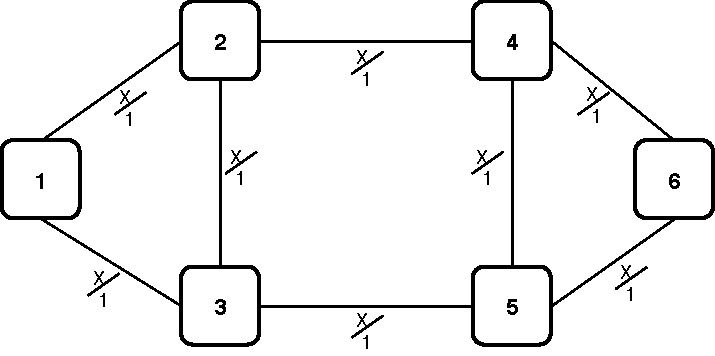
\includegraphics[width=12cm]{sdf/ilp/opaque_survivability/figures/allowed_physical_topology}
\caption{Allowed Physical Topology. The allowed physical topology is defined by the duct and sites in the field. It is assumed that each duct supports up to 1 bidirectional transmission system and each site supports up to 1 node.}
\label{allowed_physical_high}
\end{figure}

\begin{figure}[h!]
\centering
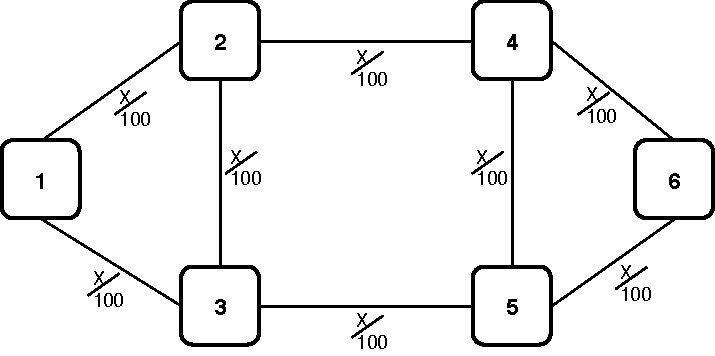
\includegraphics[width=12cm]{sdf/ilp/opaque_survivability/figures/allowed_optical_topology}
\caption{Allowed Optical Topology. The allowed optical topology is defined by the transport mode (opaque transport mode in this case). It is assumed that each transmission system supports up to 100 optical channels.}
\label{allowed_optical_high}
\end{figure}
\newpage
\begin{figure}[h!]
\centering
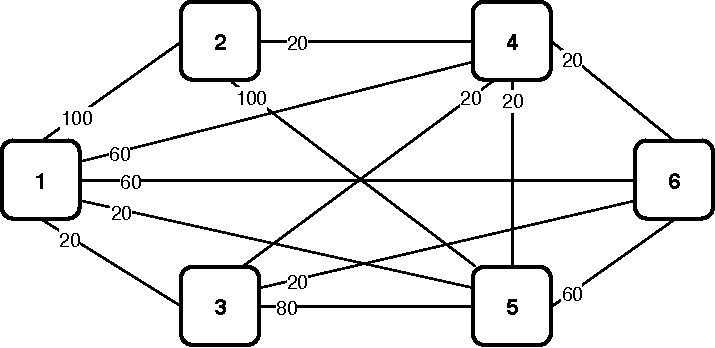
\includegraphics[width=12cm]{sdf/ilp/opaque_survivability/figures/logical_topology_ODU0_high}
\caption{ODU0 Logical Topology defined by the ODU0 traffic matrix.}
\label{logical_ODU0_high}
\end{figure}

\begin{figure}[h!]
\centering
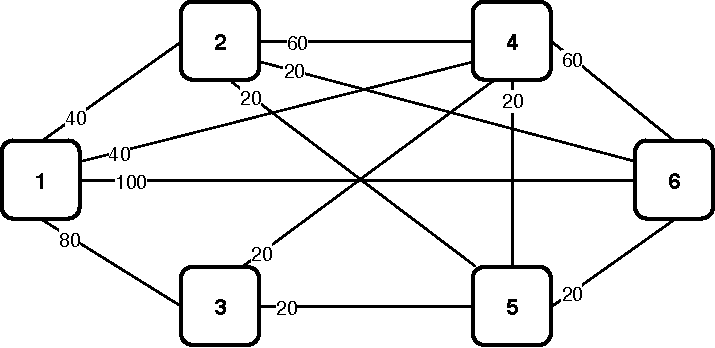
\includegraphics[width=12cm]{sdf/ilp/opaque_survivability/figures/logical_topology_ODU1_high}
\caption{ODU1 Logical Topology defined by the ODU1 traffic matrix.}
\label{logical_ODU1_high}
\end{figure}

\begin{figure}[h!]
\centering
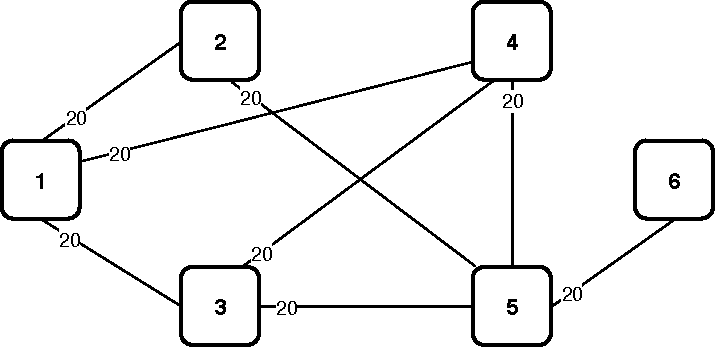
\includegraphics[width=12cm]{sdf/ilp/opaque_survivability/figures/logical_topology_ODU2_high}
\caption{ODU2 Logical Topology defined by the ODU2 traffic matrix.}
\label{logical_ODU2_high}
\end{figure}

\begin{figure}[h!]
\centering
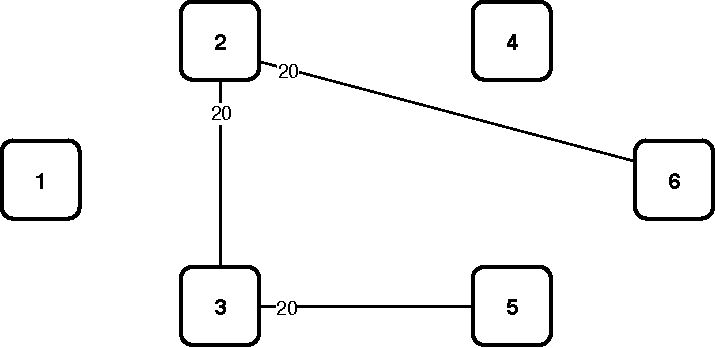
\includegraphics[width=12cm]{sdf/ilp/opaque_survivability/figures/logical_topology_ODU3_high}
\caption{ODU3 Logical Topology defined by the ODU3 traffic matrix.}
\label{logical_ODU3_high}
\end{figure}

\begin{figure}[h!]
\centering
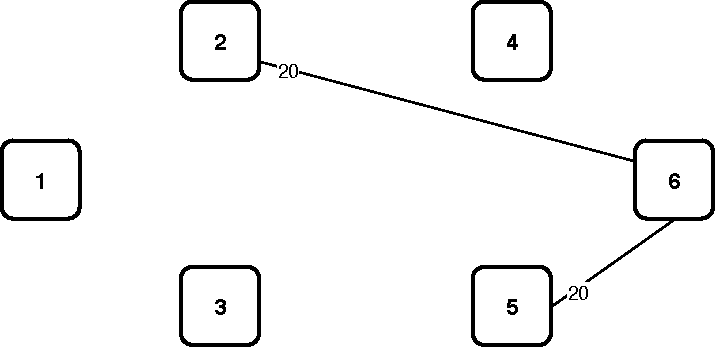
\includegraphics[width=12cm]{sdf/ilp/opaque_survivability/figures/logical_topology_ODU4_high}
\caption{ODU4 Logical Topology defined by the ODU4 traffic matrix.}
\label{logical_ODU4_high}
\end{figure}

\begin{figure}[h!]
\centering
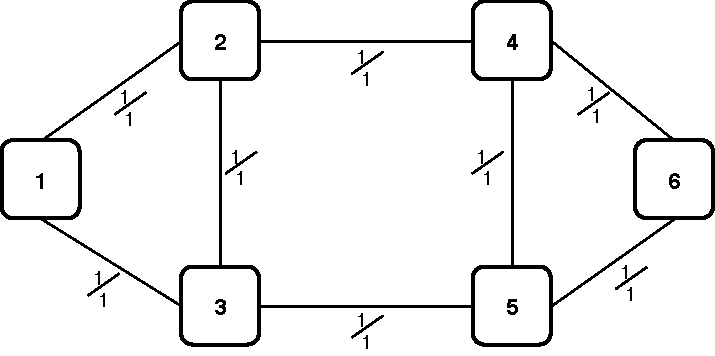
\includegraphics[width=12cm]{sdf/ilp/opaque_survivability/figures/physical_topology}
\caption{Physical Topology after dimensioning.}
\label{physical_high}
\end{figure}

\begin{figure}[h!]
\centering
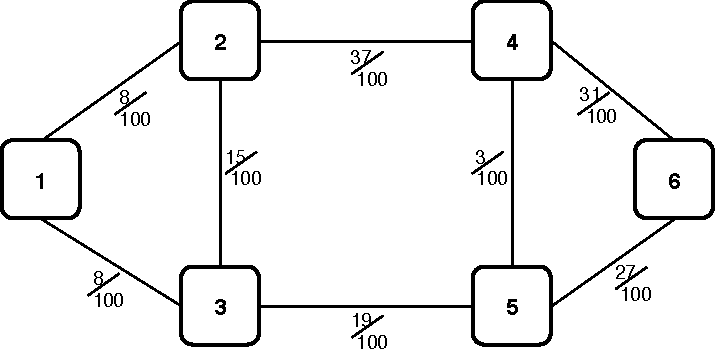
\includegraphics[width=12cm]{sdf/ilp/opaque_survivability/figures/optical_topology_high}
\caption{Optical Topology after dimensioning.}
\label{optical_high}
\end{figure}


\vspace{20pt}
In table \ref{link_opaque_surv_ref_high} we can see the number of optical channels calculated using \ref{Capex_Link} and \ref{Capex} and the number of amplifiers for each link calculated using \ref{amplifiers}.\\

\begin{table}[h!]
\centering
\begin{tabular}{|| c | c | c ||}
 \hline
 \multicolumn{3}{|| c ||}{Information regarding links} \\
 \hline
 \hline
 Bidirectional Link & Optical Channels & Amplifiers\\
 \hline
 Node 1 <-> Node 2 & 8 & 4 \\
 Node 1 <-> Node 3 & 8 & 6 \\
 Node 2 <-> Node 3 & 15 & 0 \\
 Node 2 <-> Node 4 & 37 & 6 \\
 Node 3 <-> Node 5 & 19 & 8 \\
 Node 4 <-> Node 5 & 3 & 1 \\
 Node 4 <-> Node 6 & 31 & 7 \\
 Node 5 <-> Node 6 & 27 & 3 \\
 \hline
\end{tabular}
\caption{Table with information regarding links}
\label{link_opaque_surv_ref_high}
\end{table}

\vspace{15pt}
In table \ref{node_opaque_surv_ref_high} we can see the resulting nodal degree at the physical layer, the number of line ports and the number of tributary ports for each node.\\

In each table mentioned next with detailed information we can see how many ports are connected to a given node and its bit rate (in relation to the line ports) and how many ports are assigned to each different bit rate (in relation to the tributary ports).\\
\newpage
\begin{table}[h!]
\centering
\begin{tabular}{|| c | c | c | c ||}
 \hline
 \multicolumn{4}{|| c ||}{Information regarding nodes} \\
 \hline
 \hline
 Node & Resulting Nodal Degree & Line Ports & Tributary Ports\\
 \hline
 1 & 2 & 16 & 580 \\
 2 & 3 & 60 & 460 \\
 3 & 3 & 42 & 360 \\
 4 & 3 & 71 & 400 \\
 5 & 3 & 49 & 480 \\
 6 & 2 & 58 & 440 \\
\hline
\end{tabular}
\caption{Table with information regarding nodes}
\label{node_opaque_surv_ref_high}
\end{table}

\vspace{17pt}
\begin{table}[h!]
\centering
\begin{tabular}{|| c | c | c ||}
 \hline
 \multicolumn{3}{|| c ||}{Detailed description of Node 1} \\
 \hline
 \hline
  & Node <-- Optical Channels --> Node & bit rate \\ \hline
\multirow{2}{*}{16 line ports} & 1  <---- 8 ---->  2 & \multirow{2}{*}{100 Gbtis/s} \\
 & 1  <---- 8 ---->  3 & \\
 \hline
 \hline
  & Number of tributary ports & bit rate \\ \hline
\multirow{3}{*}{580 tributary ports} & 260 & ODU0 \\
 & 260 & ODU1 \\
 & 60 & ODU2 \\
\hline
\end{tabular}
\caption{Table with detailed description of node 1}
\end{table}

\vspace{17pt}
\begin{table}[h!]
\centering
\begin{tabular}{|| c | c | c ||}
 \hline
 \multicolumn{3}{|| c ||}{Detailed description of Node 2} \\
 \hline
 \hline
  & Node <-- Optical Channels --> Node & bit rate \\ \hline
 \multirow{3}{*}{60 line ports} & 2  <---- 8 ---->  1 & \multirow{3}{*}{100 Gbtis/s}\\
 & 2  <---- 15 ---->  3 & \\
 & 2  <---- 37 ---->  4 & \\
 \hline
 \hline
  & Number of tributary ports & bit rate \\ \hline
\multirow{5}{*}{460 tributary ports} & 220 & ODU0 \\
 & 140 & ODU1 \\
 & 40 & ODU2 \\
 & 40 & ODU3 \\
 & 20 & ODU4 \\
\hline
\end{tabular}
\caption{Table with detailed description of node 2}
\end{table}

\newpage
\begin{table}[h!]
\centering
\begin{tabular}{|| c | c | c ||}
 \hline
 \multicolumn{3}{|| c ||}{Detailed description of Node 3} \\
 \hline
 \hline
  & Node <-- Optical Channels --> Node & bit rate \\ \hline
 \multirow{3}{*}{42 line ports} & 3  <---- 8 ---->  1 & \multirow{3}{*}{100 Gbtis/s}\\
 & 3  <---- 15 ---->  2 & \\
 & 3  <---- 19 ---->  5 & \\
 \hline
 \hline
  & Number of tributary ports & bit rate \\ \hline
\multirow{4}{*}{360 tributary ports} & 140 & ODU0 \\
 & 120 & ODU1\\
 & 60 & ODU2\\
 & 40 & ODU3\\
\hline
\end{tabular}
\caption{Table with detailed description of node 3}
\end{table}

\vspace{17pt}
\begin{table}[h!]
\centering
\begin{tabular}{|| c | c | c ||}
 \hline
 \multicolumn{3}{|| c ||}{Detailed description of Node 4} \\
 \hline
 \hline
  & Node <-- Optical Channels --> Node & bit rate \\ \hline
\multirow{3}{*}{71 line ports} & 4  <---- 37 ---->  2 & \multirow{3}{*}{100 Gbtis/s}\\
 & 4  <---- 3 ---->  5 & \\
 & 4  <---- 31 ---->  6 & \\
 \hline
 \hline
  & Number of tributary ports & bit rate \\ \hline
\multirow{3}{*}{400 tributary ports} & 140 & ODU0 \\
 & 200 & ODU1 \\
 & 60 & ODU2 \\
\hline
\end{tabular}
\caption{Table with detailed description of node 4}
\end{table}

\vspace{17pt}
\begin{table}[h!]
\centering
\begin{tabular}{|| c | c | c ||}
 \hline
 \multicolumn{3}{|| c ||}{Detailed description of Node 5} \\
 \hline
 \hline
  & Node <-- Optical Channels --> Node & bit rate \\ \hline
 \multirow{3}{*}{49 line ports} & 5  <---- 19 ---->  3 & \multirow{3}{*}{100 Gbtis/s} \\
 & 5  <---- 3 ---->  4 & \\
 & 5  <---- 27 ---->  6 & \\
 \hline
 \hline
  & Number of tributary ports & bit rate \\ \hline
\multirow{5}{*}{480 tributary ports} & 280 & ODU0 \\
 & 80 & ODU1 \\
 & 80 & ODU2 \\
 & 20 & ODU3 \\
 & 20 & ODU4 \\
\hline
\end{tabular}
\caption{Table with detailed description of node 5}
\end{table}

\newpage
\begin{table}[h!]
\centering
\begin{tabular}{|| c | c | c ||}
 \hline
 \multicolumn{3}{|| c ||}{Detailed description of Node 6} \\
 \hline
 \hline
  & Node <-- Optical Channels --> Node & bit rate \\ \hline
 \multirow{2}{*}{58 line ports} & 6  <---- 31 ---->  4 & \multirow{2}{*}{100 Gbtis/s} \\
 & 6  <---- 27 ---->  5 & \\
 \hline
 \hline
  & Number of tributary ports & bit rate \\ \hline
\multirow{5}{*}{440 tributary ports} & 160 & ODU0 \\
 & 200 & ODU1 \\
 & 20 & ODU2 \\
 & 20 & ODU3 \\
 & 40 & ODU4 \\
\hline
\end{tabular}
\caption{Table with detailed description of node 6}
\end{table}

\vspace{17pt}
Now through the table \ref{scriptopaque_surv_ref_high} we can see the result of CAPEX obtained with this ILP model. In table \ref{formulas_opaque_surv_ref_low} mentioned in previous scenario we can see how all the values of the quantity column were calculated.\\

\begin{table}[h!]
\centering
\begin{tabular}{|| c | c | c | c | c | c | c ||}
 \hline
 \multicolumn{7}{|| c ||}{CAPEX of the Network} \\
 \hline
 \hline
 \multicolumn{3}{|| c |}{ } & Quantity & Unit Price & Cost & Total \\
 \hline
 \multirow{3}{*}{Link Cost} & \multicolumn{2}{ c |}{OLTs} & 16 & 15 000 \euro & 240 000 \euro & \multirow{3}{*}{148 520 000 \euro} \\ \cline{2-6}
 & \multicolumn{2}{ c |}{100 Gb/s Transceivers} & 296 & 5 000 \euro/Gb/s & 148 000 000 \euro & \\ \cline{2-6}
 & \multicolumn{2}{ c |}{Amplifiers} & 70 & 4 000 \euro & 280 000 \euro & \\
 \hline
 \multirow{9}{*}{Node Cost} & \multirow{7}{*}{Electrical} & EXCs & 6 & 10 000 \euro & 60 000 \euro & \multirow{9}{*}{29 711 800 \euro} \\ \cline{3-6}
 & & ODU0 Ports & 1 200 & 10 \euro/port & 12 000 \euro & \\ \cline{3-6}
 & & ODU1 Ports & 1 000 & 15 \euro/port & 15 000 \euro & \\ \cline{3-6}
 & & ODU2 Ports & 320 & 30 \euro/port & 9 600 \euro & \\ \cline{3-6}
 & & ODU3 Ports & 120 & 60 \euro/port & 7 200 \euro & \\ \cline{3-6}
 & & ODU4 Ports & 80 & 100 \euro/port & 8 000 \euro & \\ \cline{3-6}
 & & Line Ports & 296 & 100 000 \euro/port & 29 600 000 \euro & \\ \cline{2-6}
 & \multirow{2}{*}{Optical} & OXCs & 0 & 20 000 \euro & 0 \euro & \\ \cline{3-6}
 & & Ports & 0 & 2 500 \euro/port & 0 \euro & \\
 \hline
 \multicolumn{6}{|| c |}{Total Network Cost} & 178 231 800 \euro \\
\hline
\end{tabular}
\caption{Table with detailed description of CAPEX}
\label{scriptopaque_surv_ref_high}
\end{table}

\vspace{17pt}
Finally let's focus on the routing information. These paths are bidirectional so the path from one node to another is the same path in the opposite direction. In table \ref{path_opaque_surv_ref_high} we can see all the routing obtained for all nodes.\\
\newpage
\begin{table}[h!]
\centering
\begin{tabular}{|| c | c | c ||}
 \hline
 \multicolumn{3}{|| c ||}{Routing} \\
 \hline
 \hline
 o & d & Links \\
 \hline
 1 & 2 & \{(1,2)\} \\ \hline
 1 & 3 & \{(1,3)\} \\ \hline
 1 & 4 & \{(1,2),(2,4)\}\\ \hline
 1 & 5 & \{(1,3),(3,5)\}\\ \hline
 1 & 6 & \{(1,3),(3,5),(5,6)\}\\ \hline
 2 & 3 & \{(2,3)\}\\ \hline
 2 & 4 & \{(2,4)\}\\ \hline
 2 & 5 & \{(2,3),(3,5)\}\\ \hline
 2 & 6 & \{(2,4),(4,6)\}\\ \hline
 3 & 4 & \{(3,2),(2,4)\}\\ \hline
 3 & 5 & \{(3,5)\}\\ \hline
 3 & 6 & \{(3,5),(5,6)\}\\ \hline
 4 & 5 & \{(4,5)\}\\ \hline
 4 & 6 & \{(4,6)\}\\ \hline
 5 & 6 & \{(5,6)\}\\
 \hline
\end{tabular}
\caption{Table with description of routing}
\label{path_opaque_surv_ref_high}
\end{table}

\vspace{15pt}

\subsubsection{Conclusions}

Once we have obtained the results for all the scenarios we will now draw some conclusions about these results. For a better analysis of the results will be created the table \ref{table_comparative_opaque_surv} with the number of line ports, tributary ports and transceivers because they are important values for the cost of CAPEX, the cost of links, the cost of nodes and finally the cost of CAPEX.\\

\begin{table}[h!]
\centering
\begin{tabular}{| c | c | c | c |}
 \hline
   & Low Scenario & Medium Scenario  & High Scenario \\
 \hline\hline
 Bidirectional Links used & 6 & 8 & 8 \\ \hline
 Number of Line ports & 18 & 150 & 296 \\ \hline
 Number of Tributary ports & 136 & 1 360 & 2 720 \\ \hline
 Number of Transceivers & 18 & 150 & 296 \\ \hline
 Link Cost & 9 404 000 \euro & 75 520 000 \euro & 148 520 000 \euro \\ \hline
 Node Cost & 1 862 590 \euro & 15 085 900 \euro & 29 711 800 \euro \\ \hline
 CAPEX & \textbf{11 266 590 \euro} & \textbf{90 605 900 \euro} & \textbf{178 231 800 \euro} \\
 \hline
\end{tabular}
\caption{Table with different value of CAPEX for this case.}
\label{table_comparative_opaque_surv}
\end{table}

\newpage
Looking at the previous table we can make some comparisons between the several scenarios.

\begin{itemize}
  \item Low scenario uses less links than the other two scenarios.
  \subitem This happens because as it has low traffic it is possible to carry this traffic throughout the network without having to use all available links.
  \item Comparing the Low scenario with the others we can see that despite having an increase of factor ten (medium scenario) and factor twenty (high scenario) the same increase does not occur in the final cost (it is lower).
  \subitem This happens because the number of transceivers is smaller than expected (medium scenario would be expected 180 and high scenario would be expected 360).
  \item Comparing the Medium scenario with the High scenario we can see that the increase of the factor is double and in the final cost this factor is very close but still inferior.
  \subitem Again this happens because the number of transceivers is lower but very close to the expected (high scenario would be expected 300).
\end{itemize}

\vspace{13pt}

\subsubsection{Opens Issues}

The creation of this model for any scenario, started with some considerations and some open issues being:

\begin{itemize}
  \item Allow blocking.
  \subitem The presented model assume that the solution is possible or impossible.
  \item Allow multiple transmission system.
  \subitem The presented model for each link only supports one transmission system.
  \item Allowing multi-path routing.
  \subitem The presented model for all demands sharing the same node pairs have to follow the same path.
\end{itemize}

